\documentclass{article}
\usepackage{amsmath, amssymb}
\usepackage{tikz}
\usetikzlibrary{arrows.meta, decorations.markings}

\begin{document}

\section{Plan for Class}
\begin{enumerate}
    \item Intro to bifurcations \S 3.1
    \item Co-dimension-one phenomena
    \item Unfoldings
    \item Center manifolds \S 3.2
    \item Approximating center manifolds
    \begin{enumerate}
        \item definition
        \item center manifold theorem \S 3.2.1
        \item non-uniqueness
    \end{enumerate}
    \item Dynamics on the center manifold
\end{enumerate}

\section{Intro to bifurcations \S 3.1}

\subsection{Local bifurcations}

\subsubsection{Example 1}

Suppose $\mu$ is a parameter in the following system
\[\dot{x}=\mu -x\]
The equilibrium points are 
\[\mu=x^2\]
which suggests that when $\mu$ is negative, there are no fixed points and trajectories just got to $-\infty$. When $\mu$ is positive, we have two fixed points at $x_0=\pm\sqrt{\mu}$, where $+\mu$ is stable node and $-\mu$ is a saddle node\footnote{Did we talk about saddle nodes in 1 dimension?}.

When $\mu=0$, we have a bifurcation value and $x_0=\mu$ is a semi-stable point. Moreover, if we slightly perturb $\mu$, then the dynamics of our fixed point change: it's structurally unstable. In fact, this is how we are going to define a bifurcation value.

\textit{Definition}: A bifurcation value is a value of parameter $\mu$ for which the system is not structurally stable.

Also note that this example shows a saddle-node bifurcation.

\subsubsection{Example 2}

Now let's consider the system
\[\dot{x}=\mu x -x^2\]
where we can find the fixed points via 
\[x(\mu-x)=0\]
where the fixed points are $x=0$ and $x=\mu$.

Notice that when $\mu<0$ then $x=0$ is a stable node and $x=\mu$ is a saddle. And then when $\mu>0$, we have $x=0$ is a saddle and $x=\mu$ is a stable node. This is a transcritical bifurcation!

\subsubsection{Example 3}

Now let's consider the system
\[\dot{x}=\mu x -x^3\]
where we can find the fixed points via 
\[x(\mu-x^2)=0\]
where the fixed points are $x=0$ and $x^2=\mu$.

Now when $\mu<0$, we have one fixed point at $x=0$, which is a stable node. When $\mu>0$, then $x=0$ is unstable and the fixed points at $x^2=\mu$ are stable. This is a supercritical pitchfork bifurcation!

\subsubsection{Example 3a}

Now let's consider the system
\[\dot{x}=\mu x +x^3\]
where we can find the fixed points via 
\[x(\mu+x^2)=0\]
where the fixed points are $x=0$ and $-x^2=\mu$.

Now when $\mu>0$, we have one fixed point at $x=0$, which is a unstable. When $\mu<0$, then $x=0$ is stable and the fixed points at $x^2=\mu$ are unstable. This is a \textit{subcritical} pitchfork bifurcation!

\subsubsection{Hysteresis}

When we play around with bifurcations, we can get transitions in $\mu$ that cause the fixed points to suddenly jump. The diagram is cool, so maybe I'll include it after class. I suspect this will be on the homework.

\begin{figure}[ht]
\centering
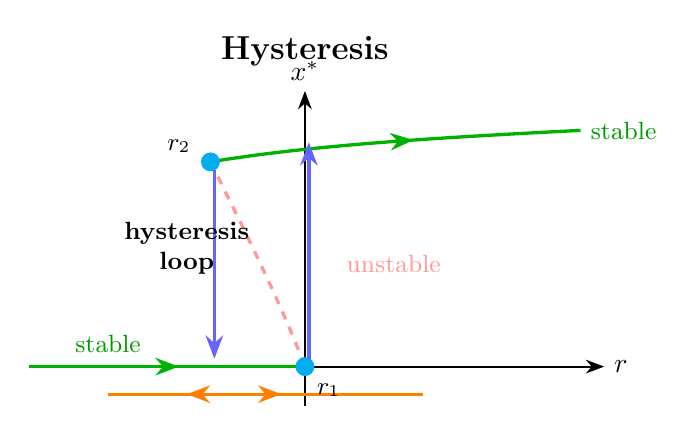
\begin{tikzpicture}[
    >=Stealth,
    thick,
    % Style for directed curves with mid-arrow
    arr/.style={
        decoration={markings, mark=at position 0.55 with {\arrow{>}}},
        postaction={decorate}
    }
]

% --- Axes ---
\draw[->] (-3.5,0) -- (3.8,0) node[right] {$r$};
\draw[->] (0,-0.5) -- (0,3.5) node[above] {$x^*$};

% --- Stable upper branch (green): from r=-1 curving up and to the right ---
% Parametric: r goes from ~-1 to 3, x^* is large positive (stable)
\draw[green!70!black, arr, very thick]
    (-1.2, 2.6) .. controls (0,2.8) and (1.5,2.9) .. (3.5, 3.0);

% --- Stable lower branch (green): the x*=0 branch for r<0 ---
\draw[green!70!black, arr, very thick]
    (-3.5, 0) -- (-0.05, 0);

% --- Unstable middle branch (pink/red, dashed): S-curve middle ---
\draw[pink!80!red, dashed, very thick]
    (-1.2, 2.6) .. controls (-0.8,1.8) and (-0.3,0.8) .. (0.0, 0.0);

% --- Saddle-node / fold point markers ---
% Left fold point (where upper stable meets unstable branch)
\filldraw[cyan] (-1.2, 2.6) circle (3pt);
% Right fold point (where unstable meets lower stable at origin vicinity)
\filldraw[cyan] (0.0, 0.0) circle (3pt) node[below right, black, font=\small] {};

% --- Hysteresis arrows on parameter axis ---
% Arrow going right (increasing r) along x-axis — jumps up
\draw[->, orange, very thick] (-2.5,-0.35) -- (-0.3,-0.35)
    node[midway, below, font=\small] {};
% Arrow going left (decreasing r) along x-axis — jumps down
\draw[->, orange, very thick] (1.5,-0.35) -- (-1.5,-0.35)
    node[midway, below, font=\small] {};

% Jump-up arrow (system jumps from x*=0 to upper branch at r=0)
\draw[->, blue!60, very thick] (0.05, 0.1) -- (0.05, 2.85);
% Jump-down arrow (system jumps from upper branch down at left fold)
\draw[->, blue!60, very thick] (-1.15, 2.5) -- (-1.15, 0.1);

% --- Labels ---
\node[green!60!black, right, font=\small] at (3.5, 3.0) {stable};
\node[pink!80!red, right, font=\small] at (0.4, 1.3) {unstable};
\node[green!60!black, above, font=\small] at (-2.5, 0.05) {stable};

% Fold labels
\node[font=\small] at (-1.6, 2.8) {$r_2$};
\node[font=\small] at (0.3, -0.3) {$r_1$};

% Hysteresis label
\node[font=\bfseries\small, align=center] at (-1.5, 1.5) {hysteresis\\loop};

% Title
\node[font=\large\bfseries] at (0, 4.0) {Hysteresis};

\end{tikzpicture}
\caption{Bifurcation diagram showing hysteresis. As the parameter $r$ increases, the system jumps up at $r_1$ to the upper stable branch. As $r$ decreases, the system only jumps back down at $r_2 < r_1$, tracing a different path — this is the hallmark of \textbf{hysteresis}. The dashed curve is the unstable branch.}
\label{fig:hysteresis}
\end{figure}

\subsection{More generally}

Say we have the system 
\[\dot{x}=f_\mu(x)\]
where $x\in\mathbb{R}^n$ and $\mu\in\mathbb{R}^k$ (this is the parameter space). Say we have a fixed point $x_0$ for some $\mu=\mu_0$ where 
\[f_{\mu_0}(x_0)=0\]
What if we change $\mu$ a little? How can we say what happens? Sometimes we get bifurcations, other times we don't.

\subsubsection{Inverse/implicit function theorem}

For $f_{\mu_0}(x_0)=0$, we can find a family of fixed points $x=g(\mu)$ for $\mu$ near $\mu_0$ and $x$ near $x_0$ as long as $D_xf_{\mu_0}(x_0)$ is invertible. This is because
\[ g'(\mu_0)=D_xf_{\mu_0}(x_0)^{-1}\cdot D_uf_{\mu_0}(x_0)\Big|_{\mu=\mu_0}\]

What $D_xf_{\mu_0}(x_0)$ being invertible implies is that there are no eigenvalues equal to 0. In fact, $D_xf_{\mu_0}(x_0)$ is invertible if and only if there are no eigenvalues equal to 0.

Kinda spaced out here so I'm confused what this gives us.

\subsection{Other types of bifurcations}

Say we have 
\[\dot{x}=\mu^2 x + x^3\]
then we have fixed points at $0=x(\mu^2+x^2)$. The only change in stability we get is at $\mu=0$ where the unstable node at $x=0$ changes to being stable. This is very degenerate since it is a bifurcation at a point. This is not our ``usual'' type of bifurcation and we want to develop tests to rule it out.

\subsection{Global bifurcations}

Say we have the system 
\begin{align*}
    \dot{x}&=y\\
    \dot{y}&= x-x^2+\mu y
\end{align*}
At $\mu=0$, we have a saddle at the origin $(0,0)$ with a homoclinic orbit and a center at $(1,0)$. When $\mu<0$, then the homoclinic orbit breaks and we have a spiral sink at $(1,0)$. When $\mu>0$, the homoclinic orbit also breaks and we have a spiral source at $(1,0)$.

Now let's look at the Jacobian of the system. We can write 
\[
Df=\begin{bmatrix}
    0 & 1 \\
    1-2x & \mu
\end{bmatrix}
\]
At $(0,0)$, the trace of $Df$ equals $\mu >0$ and the determinant equals $-1$; hence, it is a saddle node for all values of $\mu$. At $(1,0)$, the trace is $\mu$ and the determinant is $1$; hence, changing $\mu$ changes the stability of $(1,0)$. What this shows is that some features of the bifurcation are not local. The saddle node doesn't change, but it's homoclinic orbit breaks. This is a hallmark of global bifurcations and we will develop tools to talk about them.

\section{Co-dimension-one phenomena}
In $\mathbb{R}^n$, a subspace has ``co-dimension $k$'' if and only if it has dimension $n-k$.

In space of $C^1$ vector fields, we can still have a co-dimension of $1$ subspace. The example being a $C^1$ vector field with a zero eigenvalue.

The idea is that if we have $k$ params, we expect to only encounter co-dimension-$k$ phenomena.

For co-dimension one vector fields, we have two possibilities
\begin{enumerate}
    \item simple zero eigenvalues
    \begin{enumerate}
        \item Saddle-node
        \item transcritical
        \item pitchfork
    \end{enumerate}
    \item simple pure imaginary pair eigenvalues
    \begin{enumerate}
        \item Hopf bifurcation 
    \end{enumerate}
\end{enumerate}
For co-dimension two vector fields, there are three phenomena
\begin{enumerate}
    \item double zero eigenvalues, non-diagonalizable
    \begin{enumerate}
        \item Bogdanov–Takens bifurcation
    \end{enumerate}
    \item simple zero and simple pure imaginary pair 
    \begin{enumerate}
        \item zero-Hopf 
    \end{enumerate}
    \item two distinct pure imaginary pairs
    \begin{enumerate}
        \item double Hopf
    \end{enumerate}
\end{enumerate}

\section{Unfoldings}

\textit{Definition:} A universal unfolding is a family of vector fields (or maps) in the neighborhood of the structurally unstable system that contains all possible (structurally stable and ``less degenerate'') small perturbations.

\subsection{Example}
Consider the system 
\[
\dot{x}=\mu x -x^2
\]
At $\mu=0$, we have $\dot{x}=-x^2$ and then we can make a universal unfolding by writing 
\[ \dot{x}=\mu_0 + \mu x -x^2 \]
where $\mu_0$ is our ``small perturbation''. For 
\[f(x)=\mu_0 + \mu x -x^20\]
we can use the quadratic formula to write 
\[
x=\frac{-\mu\pm\sqrt{\mu^2+4\mu_0}}{-2}
\]
For $\mu_0>0$, we have two real roots (fixed points) for all values of $\mu$. For $\mu_0<0$, we have two real roots, except when $\mu^2<-4\mu_0$ where we have no real roots.

\subsection{Reducing parameters}

Generally, the universal unfolding can be hard to reason about. For 
\[
\dot{x}=-x^3
\]
our universal unfolding looks like 
\[
\dot{x}=a+bx+cx^2-dx^3
\]
where we can reduce parameters to write 
\[
\dot{x}=\bar{a}+\bar{b}x-x^3
\]
which is still a universal unfolding and is easier to reason about.

\section{Center manifold \S 3.2}

\textit{Definition:} A center manifold is an invariant manifold tangent to the center eigenspace.

Think back to the lecture on the stable and unstable manifold to reground our intuition. Unlike with the stable and unstable manifold, we can't cay anything about the behavior of the center manifold as $t\to+\infty$ or $t\to-\infty$.

This implies that unlike stable and unstable manifolds, the center manifold may not be unique.

\subsection{Example}

Let's consider the system 
\begin{align*}
    \dot{x}&=x^2\\
    \dot{y}&=-y
\end{align*}
where $x=0$ and $y=0$ are invariant manifolds. For the linearization, we get 
\[
\begin{bmatrix}
    0 & 0\\
    0 & -1
\end{bmatrix}
\]
where the center manifold is $E^c=$x axis; however, there are many trajectories in the flow field that intersect with the center manifold. This causes the non-uniqueness problem.

\subsection{Center manifold theorem}

For $\dot{x}=f(x)$, $f$ is $C^r$, and eigenspaces $E^s,E^u,E^c$ (which are eigenvectors of $Df(x_0)$), there exists invariant manifolds $W^s,W^u,W^c$ tangent to the eigenspaces where $W^s,W^u$ are $C^r$ and unique, and $W^c$ is $C^{r-1}$ and not-unique.

\subsection{Example (p. 132)}

 


\end{document}